\chapter{First chapter}
\section{Challenges and Risk Analysis}
\begin{colortable}{Risk Management Table}
	\textbf{Risks} & \textbf{Date of Identification}  & \textbf{Date of Resolution}  & \textbf{Method of Resolution} \\ \hline
	Finding a DBMS technology that is able to process the specified number of operations & 2/12/18 & 17/12/18 & Decided on a hybrid embedded database (using an interactive query and a high throughput DBMS e.g. RocksDB or something of similar calibre).\\ \hline
	Message broker support for the AMQP protocol & 2/12/18 & 17/12/18 & Swapped AMQP for the Kafka messaging protocol. \\ \hline 
	Finding a Network protocol that can handle the 10Mb message load & 2/12/18 & 17/12/18 & Decided on the Kafka binary protocol over TCP. \\ \hline  
\end{colortable}
\newpage
\section{Requirements Refinement}
\subsection{Functional Requirements}
\subsubsection{Dashboard requirements}
\begin{itemize}
    \item \textbf{Dashboard-Queries}: The dashboard allows the user to perform queries on the data provided by the system's tools, after they have been stored in the analytics database. 
    \item \textbf{Dashboard-Filters}: The user can use filters that apply constraints on the queries.
    \item \textbf{Dashboard-Default}: The dashboard has an initial mode in which it performs a default query upon initialization.
\end{itemize}

\subsubsection{Database Requirements}
\begin{itemize}
    \item \textbf{Information-Structure}: The database system should allow for storage of structured information about a specific tool.
    \item \textbf{Information-Concurrency}: The database system should allow for concurrent operations like selection, update and insertion.
    \item \textbf{Information-Processing}: The database system stores information about tools after they have been processed with additional predefined data provided by another system.
\end{itemize}

\subsubsection{Input/Output Requirements}
\begin{itemize}
    \item \textbf{IO-Input}: The system should be able to capture information from the tools in real time.
    \item \textbf{IO-Output}: The system should provide the processed information in real time.
\end{itemize}
\newpage
\subsection{Non-Functional Requirements}
\begin{itemize}
    \item \textbf{Scalability:} \begin{itemize}
        \item The system needs to be able to support a volume of data with peaks of 80000 messages per 30 minutes.
        \item The system needs to be able to scale up to a volume of data with peaks of 160000 messages per 30 minutes.
    \end{itemize}
    \item \textbf{Performance}: \begin{itemize}
        \item The system should be able to handle an amount of data of up to 10Mb per message.
        \item The system should guarantee that the time period from a message broadcast until the storage of the message in the analytics database is less or equal to 5 minutes.
    \end{itemize}
    \item \textbf{Availability}: The system should guarantee High Availability of class 5, which means Uptime should be 99,999\% and downtime should be less or equal to 5.25 minutes per year.
    \item \textbf{Reliability}: The system needs to be fault tolerant, the system architecture should be without Single Points of Failure.
\end{itemize}
\subsection{Requirements Prioritization}
Each requirement is given a priority on a scale of 1 to 5, with value of 1 indicating a minimum priority and a value of 5 indicating a maximum priority.\\
\subsubsection{Priorities of Functional Requirements}
\begin{itemize}[nosep]
    \item Dashboard-Queries: 4
    \item Dashboard-Filters: 3
    \item Dashboard-Default: 5
    \item Information-Structure: 5
    \item Information-Concurrency: 5
    \item Information-Processing: 5
    \item IO-Input: 5
    \item IO-Output: 5
\end{itemize}
\newpage
\subsection{Use-Case Diagrams}
The team has identified the following actors in the system:
\begin{itemize}
    \item User
    \item Tool
    \item System
\end{itemize}

\subsubsection{User use case diagram}
\begin{figure}[H]
\centering
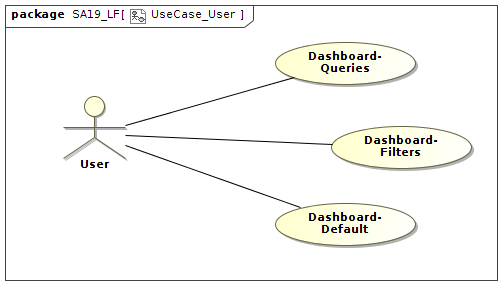
\includegraphics[width=\textwidth]{img/UseCase_User.png}
\caption{Use case diagram of the actor \textbf{User}.}
\end{figure}

\subsubsection{Tool use case diagram}
\begin{figure}[H]
\centering
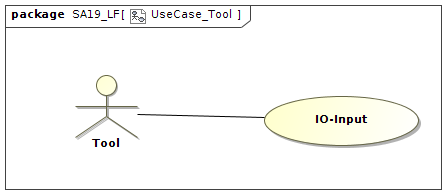
\includegraphics[width=\textwidth]{img/UseCase_Tool.png}
\caption{Use case diagram of the actor \textbf{Tool}.}
\end{figure}

\subsubsection{System use case diagram}
\begin{figure}[H]
\centering
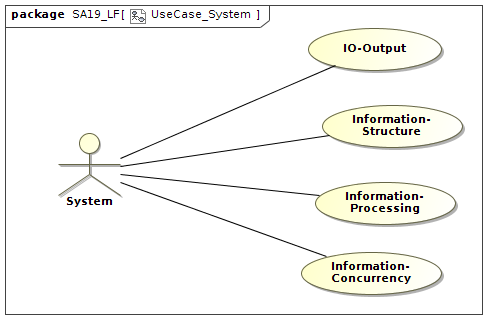
\includegraphics[width=\textwidth]{img/UseCase_System.png}
\caption{Use case diagram of the actor \textbf{System}.}
\end{figure}

\subsection{Tabular description of the most important requirements}
\begin{table}[H]
\caption{Information-Processing table}
\begin{tabular}{ |c|c| }
				\hline
 				\textbf{Use case name} & Information-Processing  \\
 				\hline
 				\textbf{Participating actors} & Tools, External system, system  \\
 				\hline
  				\textbf{Description} & 
      				\begin{tabular}{c}
      				     After that the system has collected \\
      				     the information sent by a tool,\\
      				    it processes it adding data, \\
      				    and stores it into the database system
      				\end{tabular} \\ 
 				\hline
 				\textbf{Triggering event} & Information receiving \\ 
 				\hline
 				\textbf{Priority} & High, level 5 \\ 
 				\hline
\end{tabular}
\end{table}
\begin{table}[H]
\caption{IO-Input table}
\begin{tabular}{ |c|c| } 
				 \hline
 				\textbf{Use case name} & IO-Input  \\
 				\hline
 				\textbf{Participating actors} & Tools, system  \\
 				\hline
  				\textbf{Description} & 
      				\begin{tabular}{c}
      				     Whenever a tool sends information, \\
      				     the system has to capture it in any case\\
      				\end{tabular}\\ 
 				\hline
 				\textbf{Triggering event} & Information receiving \\ 
 				\hline
 				\textbf{Priority} & High, level 5 \\ 
 				\hline
\end{tabular}
\end{table}
\begin{table}[H]
\caption{Dashboard-Default table}
\begin{tabular}{ |c|c| } 
				 \hline
 				\textbf{Use case name} & Dashboard-Default  \\
 				\hline
 				\textbf{Participating actors} & User, system  \\
 				\hline
  				\textbf{Description} &
      				\begin{tabular}{c}
      				     	Whenever the user execute the dashboard, \\
          				    the system should prints a default query
          			\end{tabular}\\ 
 				\hline
 				\textbf{Triggering event} & Dashboard request \\ 
 				\hline
 				\textbf{Priority} & Medium-High, level 4 \\ 
 				\hline
\end{tabular}
\end{table}

\section{Informal Description of the System \& its Software Architecture}

\subsection{Description of the System}

The system is composed of different high level components:
\begin{itemize}
    \item \textbf{fab\textunderscore data connector}: Under the assumptions described in the section \ref{first_design_decision}, we get the events from the database fab\textunderscore data. So the purpose of this component is to constantly query the external database in order to insert these information into our system. The method used to stream from the fab\textunderscore data database is described in \ref{kafka_connect}.
    
    \item \textbf{raw\textunderscore data connector}: The purpose of this component is to query external raw\textunderscore data database in order to retrieve the 10Mb files that contain the recipe regarding a specific tool. The method used to stream from the raw\textunderscore data database is described in \ref{kafka_connect}.
    
    \item \textbf{Message Broker}: This is the main component of our system: it takes the information from  both the \textbf{fab\textunderscore data connector} component and the \textbf{raw\textunderscore data connector}, manipulates them and performs message translation \& processing.  After the computation, this component stores its results in the \textit{analytics\textunderscore database}\\
    It also manages the information that the final users can monitor in the dashboard after applying the selected filters, The result information are retrieved from the \textit{analytics database}.
    
    \item \textbf{Analytics Database}: This the component responsible for the storage of the information. It contains the database itself but also DBMS and a controller used to perform storage operations (insertion,selection, etc). When the user apply specific filters in the dashboard these information has to be retrieved in this component's database.
\end{itemize}

\subsection{Architectural Pattern}
The team has decided to use \textbf{Publish/Subscribe} pattern, major information are in \ref{second_design_decision}.

\subsection{System boundaries}
External Components:
\begin{itemize}
    \item The database raw\textunderscore data is provided by the customer and so are the information regarding the recipes. The database is assumed to be reliable and fault tolerant. Also the information stored in it are assumed to be consistent and updated in real time. This system will be simulated in our prototype but without their non-functional requirements.
    \item The database fab\textunderscore data is provided by the customer and so are the information regarding the tools event. The database is assumed to be reliable and fault tolerant. Also the information stored in it are assumed to be consistent and updated in real time. This system will be simulated in our system prototype but without their non-functional requirements.
    \item A \textbf{network} with an architecture that is able to support the needed ratio of information. 
\end{itemize}

\subsection{Informal Diagram of the System}

\begin{figure}[H]
\centering
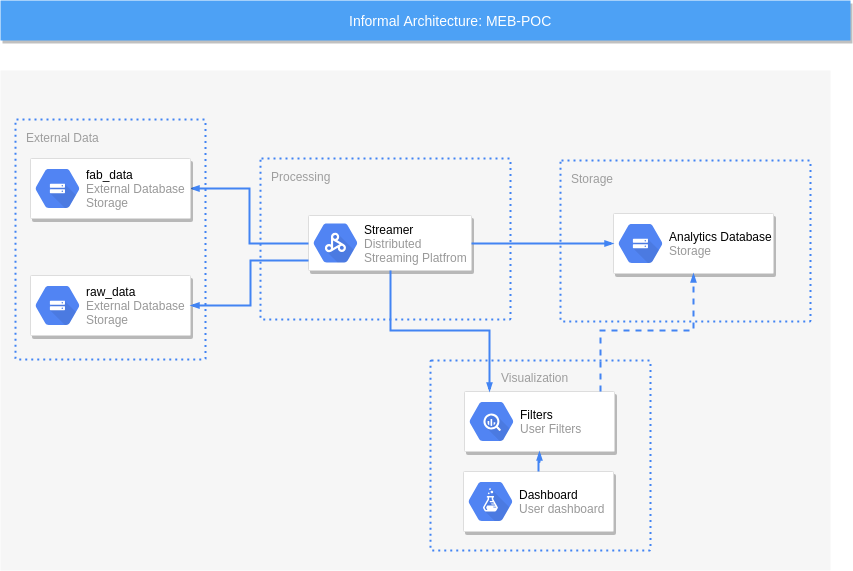
\includegraphics[width=\textwidth]{img/InformalDiagram.png}
\caption{Informal architecture of the system.}
\end{figure}

\subsection{Requirements' Fulfillment}
The requirements have been fulfilled in the following way:
\begin{itemize}
    \item \textbf{Dashboard-Queries}: The dashboard allows the user to perform queries on the data provided by the system's tools. There are two major REST endpoint, one \textit{/category/{n}} allows the user to get all the information regarding the category number {n}, the other \textit{/tool/{eqipID}} allows the user to get all the information about a specific tool identified by equipID. 
    \item \textbf{Dashboard-Filters}: The user has the possibility to apply filters.
    \item \textbf{Dashboard-Default}: The dashboard has an initial mode in which it will perform a default query.
    \item \textbf{Information-Structure}: The database system allows the storage of structured information about a specific tool into the Analytics database by using both a DBMS and the Kafka Embedded Database.
    \item \textbf{Information-Concurrency}: The database system allows concurrent operations like selection, update and insertion by using a JDBC specific driver.
    \item \textbf{Information-Processing}: The database system stores information about tools after they have been processed with additional predefined data provided by another system.
    \item \textbf{IO-Input}: The system is able to capture information from the tools in real time by using the interface to fab\_data and raw\_data databases which will publish the required information to their specific topics.
    \item \textbf{IO-Output}: The system provides the processed information in real time.
     \item \textbf{Scalability}: This is provided by the message broker.
    \item \textbf{Performance}:  The system is able to handle both the amount of requests and data as stated in the requirements.
    \item \textbf{Availability}: The developed system does respect this requirement.
    \item \textbf{Reliability}: The system architecture and the prototype are without Single Points of Failure. One tool that helps us in fulfilling this goal is the message broker that provides redundancy and fault tolerance.
\end{itemize}


\section{Design decisions}


\subsection{Tools' events (fab\_data capture) - fetching from DBMS vs sensor interception}
\label{first_design_decision}
  
    \begin{figure}[H]
\centering
 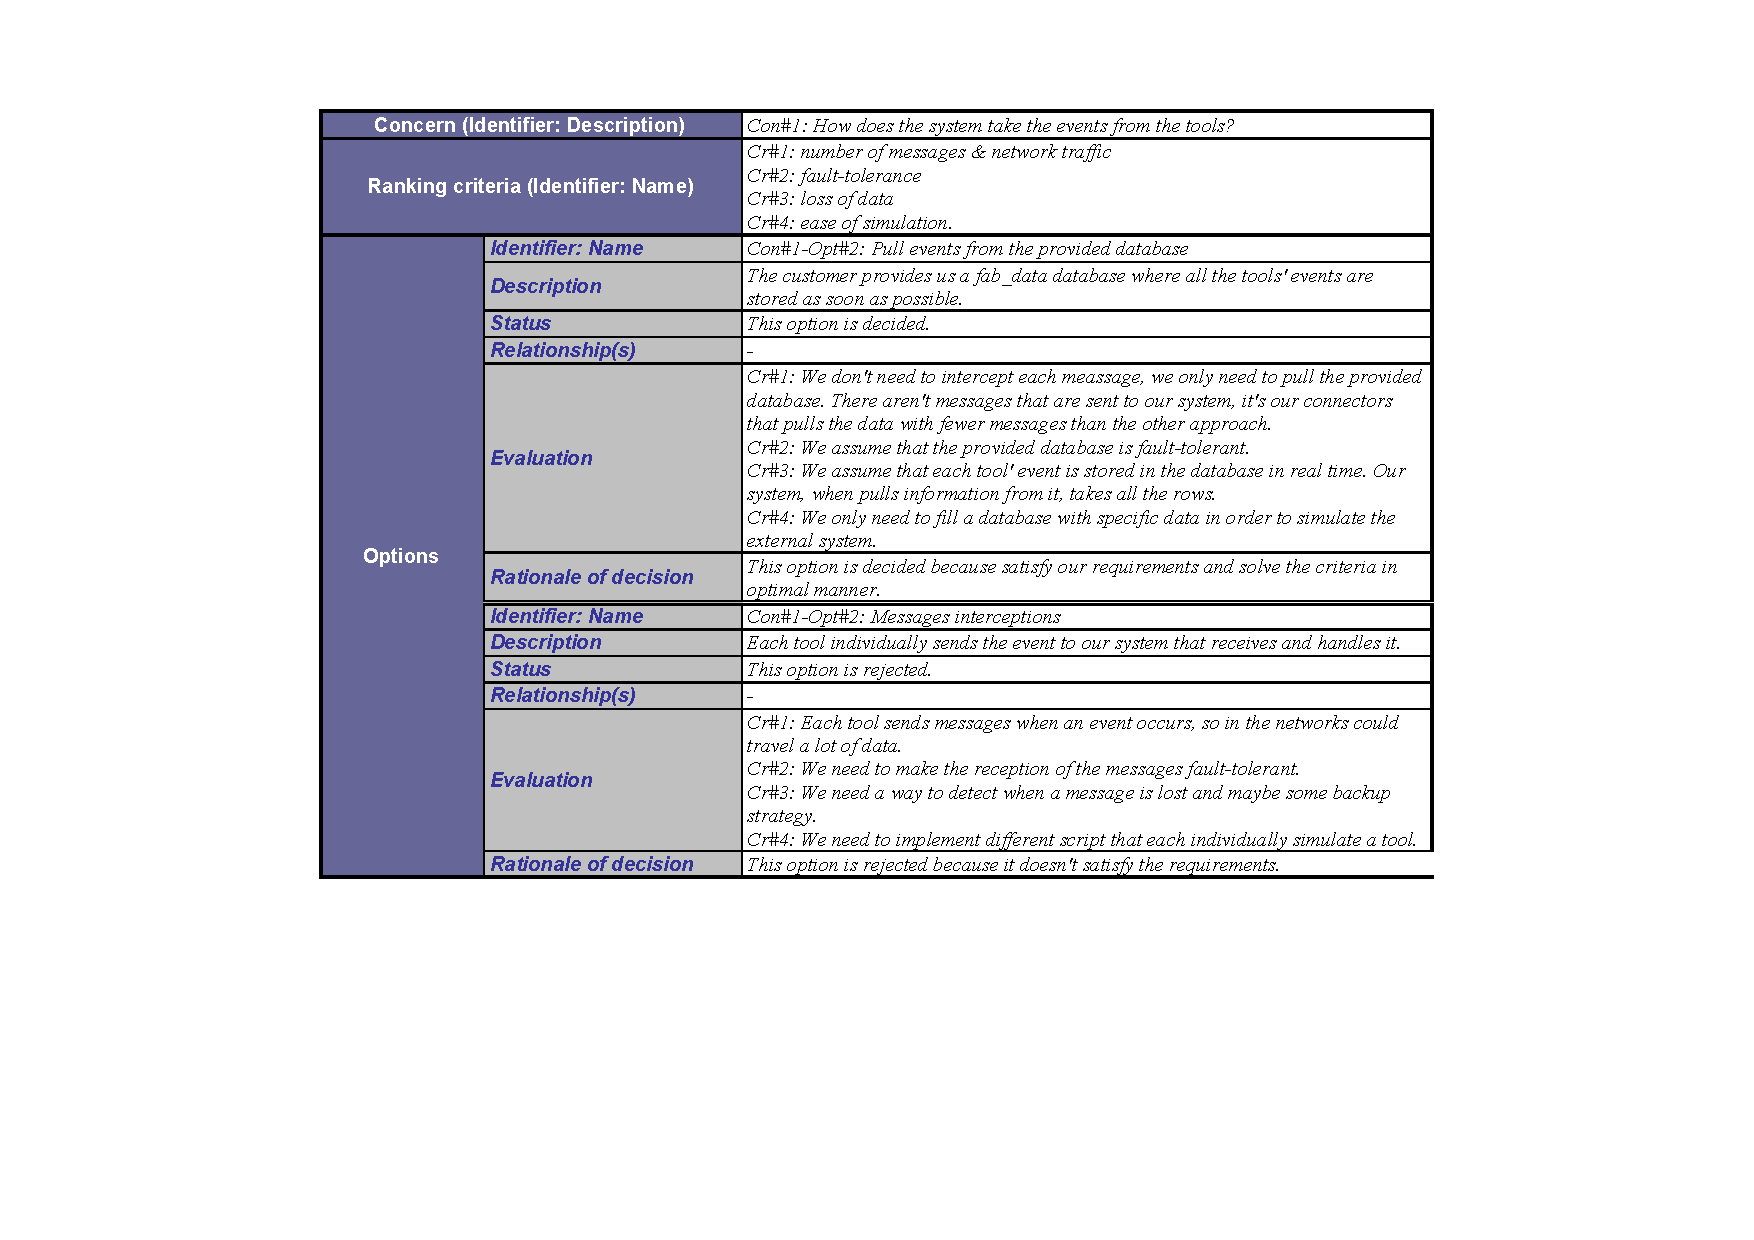
\includegraphics[trim=5cm 5.5cm 5cm 1cm,clip=true, width=\textwidth]{dd/dd1.pdf}
\caption{First design decision.}
\end{figure}
In order to prevent an high amount of messages towards our system which would be hard and time-consuming to manage individually, the team has decided to obtain the tools’ data from the \textit{fab\textunderscore data} database, which is provided externally.

The team assumes that the provided \textit{fab\textunderscore data} database is fault-tolerant and that the information are stored in it as soon as they are made available by their generating tools (in real-time).

This choice prevents loss of data in case of problems in the system’s connection, guarantees that every message will be retrieved by the system, makes it possible to eventually rebuild the history of messages.

\newpage
\subsection{Architectural Pattern}
\label{second_design_decision}
 \begin{figure}[H]
\centering
 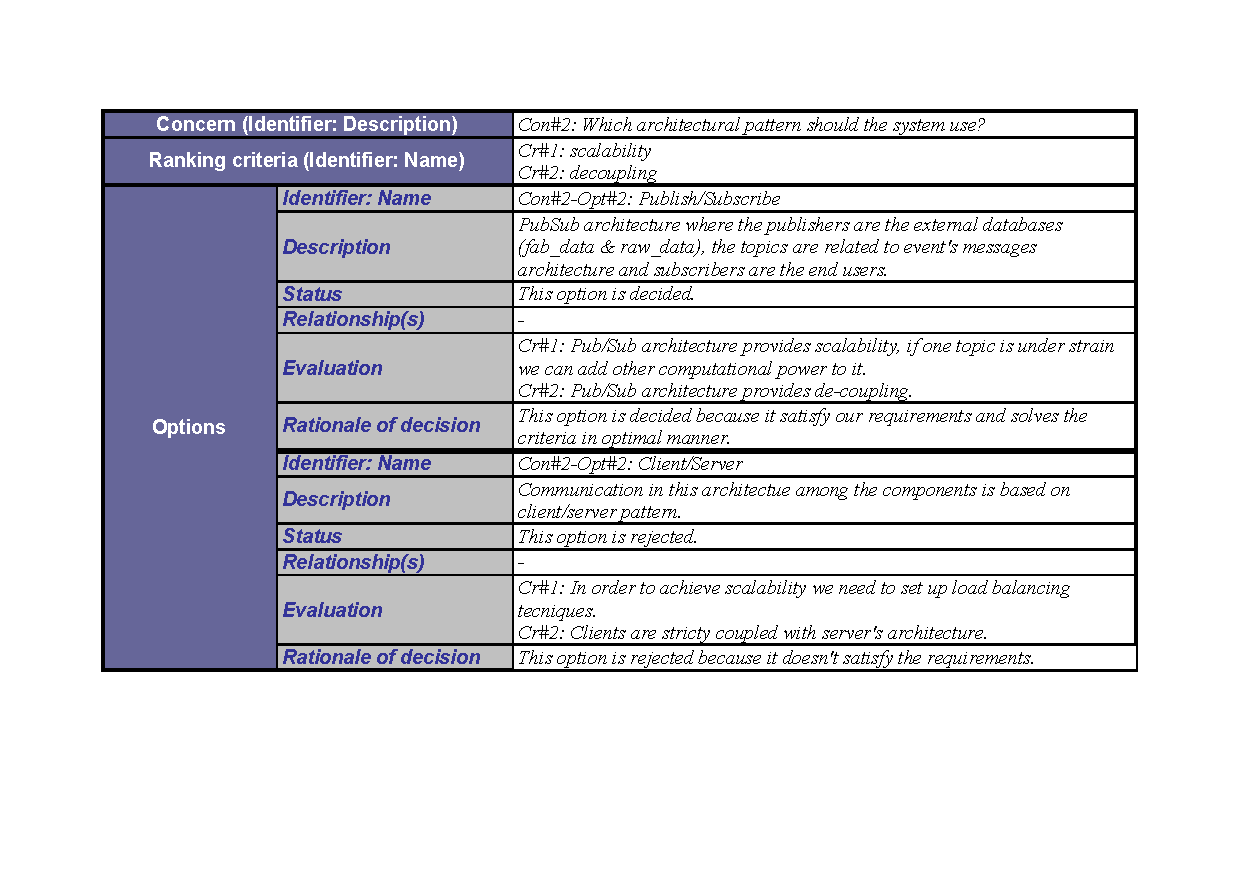
\includegraphics[trim=1.5cm 3cm 1.5cm 1.3cm,clip=true, width=\textwidth]{dd/dd2.pdf}
\caption{Second design decision.}
\end{figure}
The team has decided to opt for a Publish/Subscribe architecture. 
In the context of our application the publisher of the messages (i.e. the \textbf{producer}) is the component that gets the information from the \textit{fab\textunderscore data} database. So the messages of the system are the tools event (whose structure is described in the project specification). 
The \textbf{consumers} of the system are the users and the topics are the different categories. Components may subscribe to a set of events. It is the job of the publish-subscribe run-time infrastructure to make sure that each published event is delivered to all subscribers on that category.

We have decided to use this architectural pattern also because
Publish/Subscribe has great \textbf{scalability}, if we see that the current system is unable to satisfy our system constraints we can identify the most computationally loaded topics and subscribe other servers to these topics in order to parallelize their work (\textbf{horizontal scalability}). 
Another advantage is the \textbf{decoupling} of the system, publishers are loosely coupled to subscribers and so they are allowed to remain ignorant of system topology.


\subsection{From Message Broker to Streaming Platform}
\label{third_design_decision}

 \begin{figure}[H]
\centering
 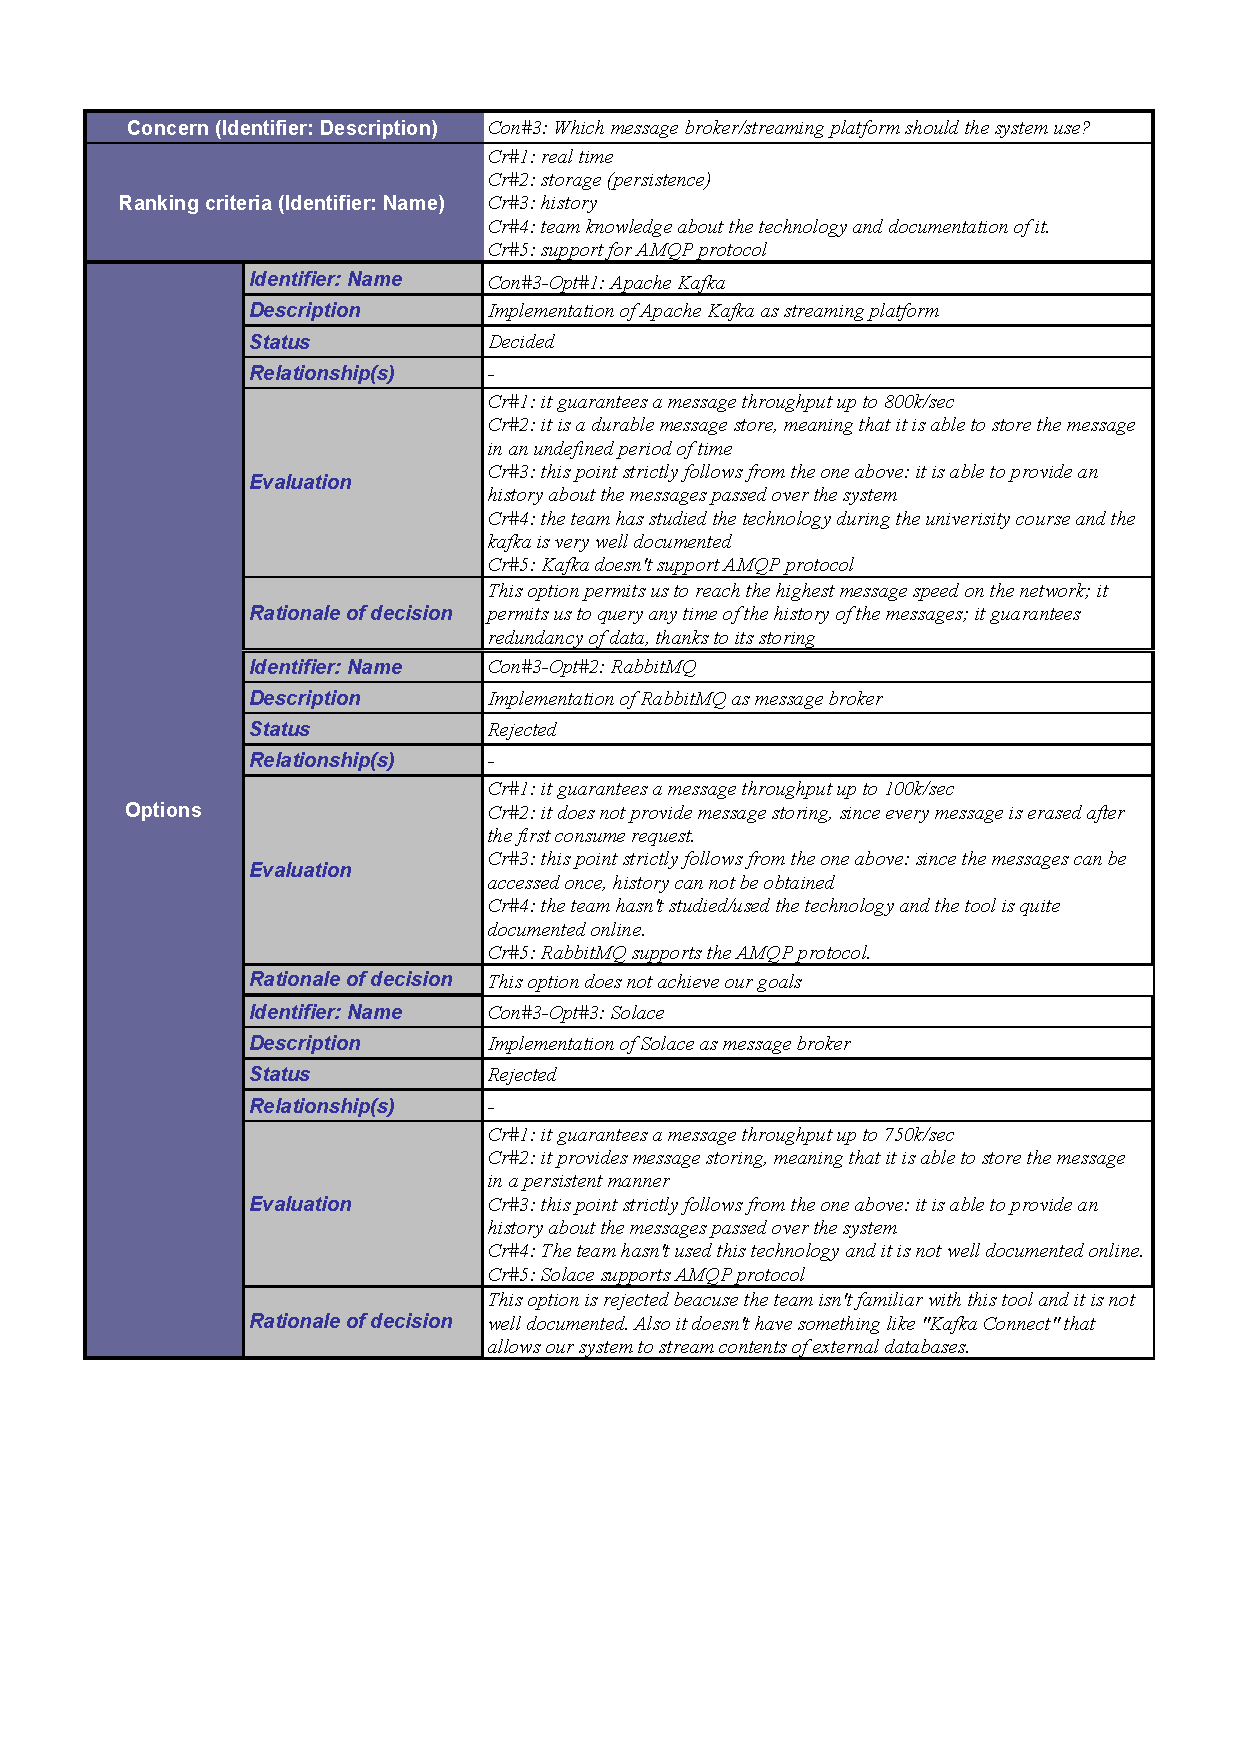
\includegraphics[trim=1cm 6.5cm 1cm 1.3cm,clip=true, width=\textwidth]{dd/dd3.pdf}
\caption{Third design decision.}
\end{figure}
\subsubsection{Apache Kafka}
In order to manage the messages, the team has decided to implement the Apache Kafka \textbf{Streaming Platform} instead of a conventional message broker.
Kafka perfectly complies with our needs\footnote{\url{https://content.pivotal.io/blog/understanding-when-to-use-rabbitmq-or-apache-kafka}}. It guarantees a very high throughput in terms of messages digested (peak of 800k/sec
\footnote{\url{https://engineering.linkedin.com/kafka/benchmarking-apache-kafka-2-million-writes-second-three-cheap-machines}}), which accomplishes our goal to afford the real time message processing. In this scenario, Kafka provides the fastest speed, compared to other message brokers like RabbitMQ, which could handle up to 100k/sec messages - due to its routing complexity.
Regarding storage, Kafka is better than RabbitMQ: Kafka is a durable message store, in which clients can get a \textit{replay} of the event stream on demand, as opposed to more traditional message brokers where once a message has been delivered, it is removed from the queue.
In our case this feature is useful since it permits to achieve a history of the messages which have passed through the system, and a recovery plan in case of malfunction, since Kafka permits the storage of the data.

\subsubsection{Kafka Connect}
\label{kafka_connect}
Another reason that favors Kafka over other Message Borker is Kafka Connect API\footnote{\url{https://docs.confluent.io/current/connect/index.html}}, more specifically a \textbf{Source Connector} which could "ingest entire databases and stream table updates to Kafka topics.". This is exactly the way in which the team has decides to pull information from the external \textit{fab\textunderscore data} and \textit{raw\textunderscore data} databases.

There are also two different ways that could be used in order to implement this external database "streaming" as states in this article\footnote{\url{https://www.confluent.io/blog/no-more-silos-how-to-integrate-your-databases-with-apache-kafka-and-cdc}}, either by using a JDBC plugin for the database's driver or by using \textbf{CDC} (i.e. \textit{Log-based Change-Data-Capture}). The team has opted for the CDC, in particular by using the Debezium\footnote{\url{https://debezium.io/}} platform.

\subsection{Recipes' Retrieval - raw\_data caching}
\label{forth_design_decision}
 \begin{figure}[H]
\centering
 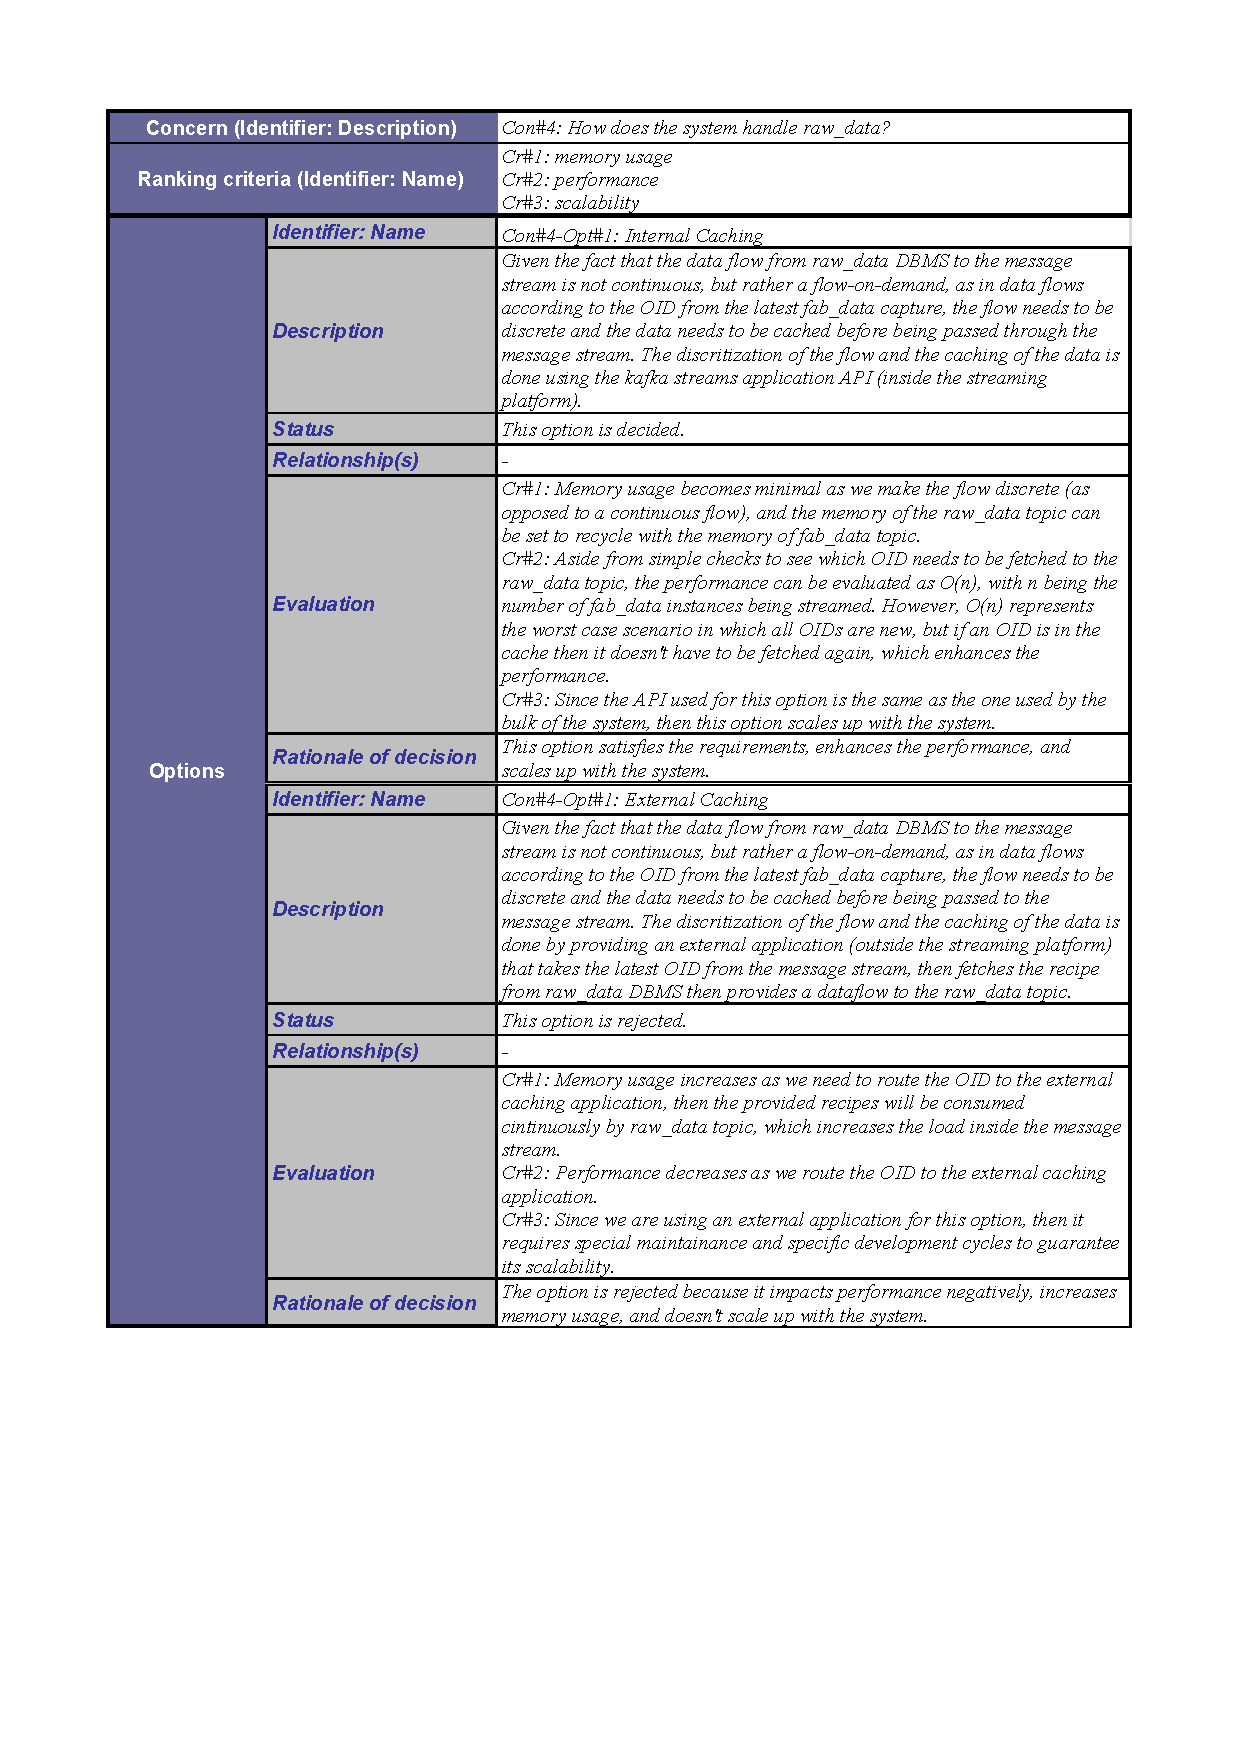
\includegraphics[trim=1.3cm 6.5cm 1.3cm 1.3cm,clip=true, width=\textwidth]{dd/dd4.pdf}
\caption{Forth design decision.}
\end{figure}

In order to integrate the process of recipe retrieval from the raw\_data DBMS, the team has decided to build an integrated discrete cashing methodology within the streaming platform using its own API.\\
This methodology allows for a dataflow-on-demand from the raw\_data DBMS only when needed, robust and interlocked development cycle, and scalability out of the box.

\subsection{Storage}
\label{firfth_design_decision}
 \begin{figure}[H]
\centering
 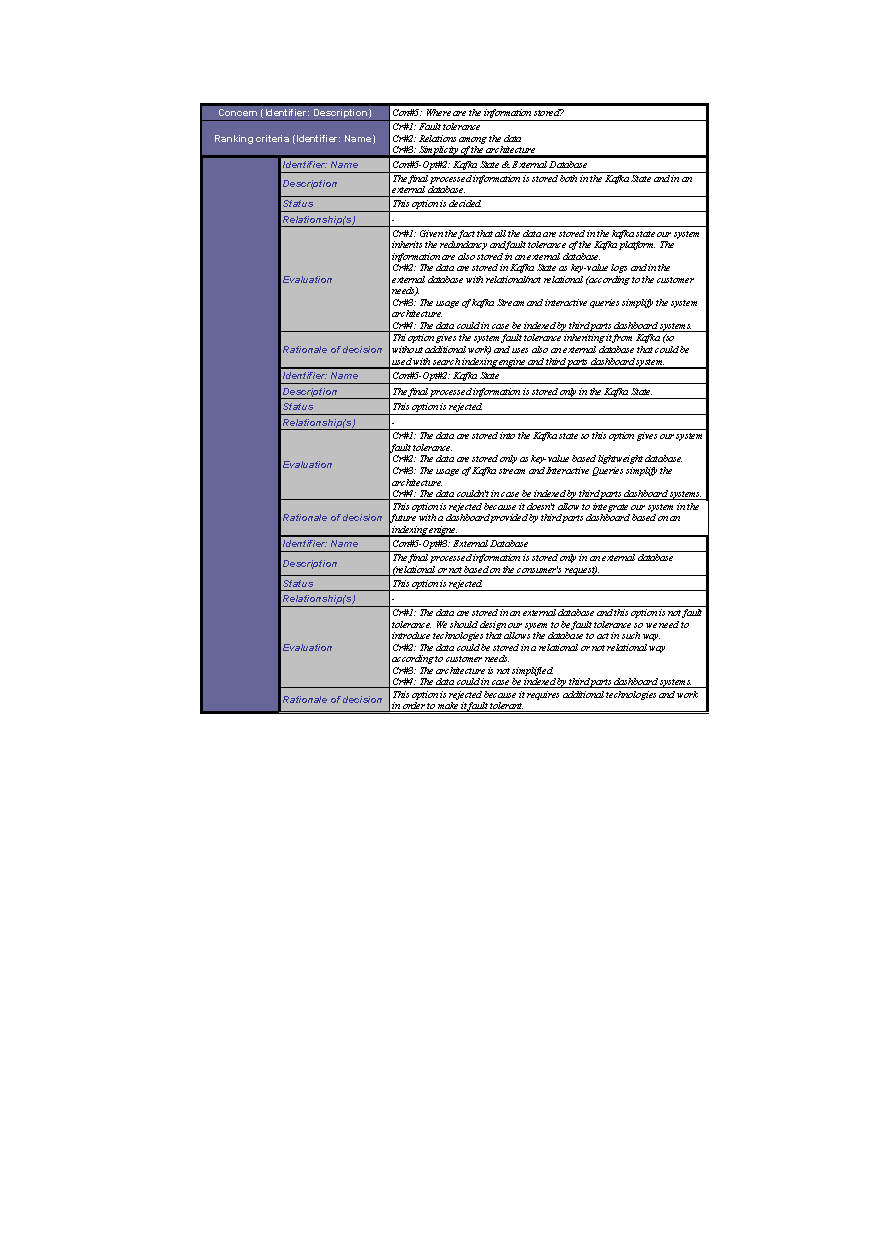
\includegraphics[trim=2.5cm 8.5cm 2.5cm 1.3cm,clip=true, width=\textwidth]{dd/dd5.pdf}
\caption{Fifth design decision.}
\end{figure}

In our system we need to store the  analytics information in a database.

In the project specification there are two constraints, our system needs to handle 80.000 messages every 30 minutes (Constraint 1) and should be able to scale up to 160.000 messages every 30 minutes (Constraint 2). So the messages flow is the following:

\begin{table}[H]
\caption{Messages ratio table}
\centering
\begin{tabular}{ |c|c|c| } \hline
\multicolumn{2}{|c|}{\textbf{Number of messages}} & \multirow{2}{2em}{\textbf{Time}} \\ \cline{1-2}
\textbf{Constraint 1} & \textbf{Constraint 2} & \\ \hline
80.000 & 160.000 & 30 min \\ \hline
$\approx2.700$ & $\approx5.200$ & 60 sec \\ \hline
$\approx45$ & $\approx 90$ & 1 sec \\ \hline
\end{tabular}
\label{table1}
\end{table}

Also the user, by using dashboard, could request both real-time and past information.
In order to provide the user with the real-time information the team has decided that the user could subscribe to the requested topics (i.e. the topics where the translated information are published).
As for the queries of past information the team has decided to use Interactive Queries provided by Apache Kafka, which makes the interrogation on kafka's logs, so they use the streaming platform also as permanent storage. This approach is discussed in the official documentation \footnote{\url{https://docs.confluent.io/current/streams/concepts.html\#interactive-queries}}.
The team has decided to store the information also in an external database (which could be relational or not relational but in our prototype we used a MongoDB's one) because in this way we could extend our system with real-time and non-real-time dashboard provided by third parts software which require traditional databases (like Kibana). 


\section{Views and Viewpoints}
\textbf{Stakeholders:}
\begin{itemize}
    \item \textbf{Sensor Engineer}: Responsible for designing and implementing the sensor networks. 
    \item \textbf{Core Developer}: Designs the communication system and the streams application (built using the streaming platform) that process our data. 
    \item \textbf{Database Developer}: Designs and administrates the database where our information are stored.
    \item \textbf{UI Designer}: Responsible for developing the dashboard where the information will be displayed.
    \item \textbf{System Integrator}: Responsible for system integration, emergency response and system migration.
    \item \textbf{End Users}: The final user of our system.
\end{itemize}
\begin{colortable}{Concern-Stakeholder Traceability}
& \textbf{\footnotesize Sensor Engineer} & \textbf{\footnotesize Core Developer} & \textbf{\footnotesize Database Developer} & \textbf{\footnotesize UI Designer} &  \textbf{\footnotesize System Integrator} & \textbf{\footnotesize End User} \\ \hline
Security &  & X & X &  & X & \\ \hline
Cost & X & X & X & X & X & \\ \hline
\footnotesize Networking \& Communication & & X & & & X & \\ \hline
Data Analysis & X & X & & & & X \\ \hline
Response Time & & X & X & & X & X \\ \hline
\makecell{ Depend-\\ ability} & X & X & X & X & X & \\ \hline
Usability &  &  &  &  &  & X \\ \hline
\makecell{Scala-\\bility} & & X & & & X & \\ \hline
Energy Consumption & X & X & & & & \\ \hline
\end{colortable}